\documentclass[11pt, a4paper]{article}
\usepackage[left=2cm,top=3cm, text={17cm,24cm}]{geometry}
\usepackage[utf8]{inputenc}
\usepackage[T1]{fontenc}
%\usepackage[czech]{babel}
\usepackage{times}
\usepackage{multirow}
\usepackage[ruled,linesnumbered]{algorithm2e}
\usepackage{algorithmic}
\usepackage{amsmath}
\usepackage{graphics}
\usepackage{picture}
\usepackage{tikz}
\usepackage{pdflscape}

\newcommand{\myuv}[1]{\quotedblbase #1\textquotedblleft}
\renewcommand{\figurename}{Obrázek}
\renewcommand{\tablename}{Tabulka}
\renewcommand{\algorithmcfname}{Algoritmus}

\SetKwInput{KwData}{Input}
\SetKwInput{KwResult}{Output}
  
\begin{document}

\begin{titlepage}
 \begin{center}
 {
  \Huge
  \textsc{Vysoké učení technické v~Brně\\
  \vspace{-2mm}
  \huge
  Fakulta informačních technologií}\\
 }
  \vspace{\stretch{0.382}}
 {
  \LARGE
  Typografie a~publikování\,--\,3. projekt\\
 }
  \vspace{-0.5mm}
 { 
  \Huge
  Tabulky a~obrázky\\
 }
  \vspace{\stretch{0.618}}
 \end{center}
{\Large 20. března 2017 \hfill Patrik Holop}
\end{titlepage}

\section{Úvodní strana}
Název práce umístěte do zlatého řezu a~nezapomeňte uvést dnešní datum a~vaše jméno a~příjmení.

\section{Tabulky}
Pro sázení tabulek můžeme použít buď prostředí \texttt{\ tabbing\ } nebo prostředí \texttt{\ tabular}.

\subsection{Prostředí \texttt{\ tabbing}}
Při použití \texttt{\ tabbing\ } vypadá tabulka následovně:

\begin{tabbing}{c|c|c}
 \qquad\qquad\quad\= 25,90\quad\= \ Množství\kill
 \bfseries Ovoce\>\bfseries \ Cena\>\bfseries \ Množství\\
 Jablka\> \ 25,90 \> \ 3 kg\\
 Hrušky\> \ 27,40 \> \ 2,5 kg\\
 Vodní melouny\> \ 35,--\> \ 1 kus\\
\end{tabbing}
Toto prostředí se dá také použít pro sázení algoritmů, ovšem vhodnější je použít 
prostředí \texttt{\ algorithm\ } nebo \texttt{\ algorithm2e\ } (viz sekce \ref{sec:sekce3}).

\subsection{Prostředí \texttt{\ tabular}}
Další možností, jak vytvořit tabulku, je použít prostředí \texttt{\ tabular}. Tabulky pak 
budou vypadat takto\footnote{Kdyby byl problém s~\texttt{\ cline}, zkuste se podívat třeba sem: http://www.abclinuxu.cz/tex/poradna/show/325037.}:


\begin{table}[h] 
 \begin{center}
 \begin{tabular}{|l|r|r|}
  \hline
  & \multicolumn{2}{|c|}{\bfseries Cena}\\ \cline{2-3}
  \bfseries Měna & \bfseries nákup & \bfseries prodej\\ \hline
  EUR & 27,02 & 27,20 \\
  GBP & 31,08 & 31,80 \\
  USD & 25,15 & 25,51 \\
  \hline
  \end{tabular}
  \\[10pt]
  \end{center} 
 \caption{Tabulka kurzů k~dnešnímu dni} 
 \label{tab:tab1}
\end{table}

\begin{table}[h] 
\begin{center}
 \begin{tabular}{|c|c|}
 \hline
 A & $\neg A$ \\ \hline
 \textbf{P} & N \\\hline
 \textbf{O} & O \\ \hline
 \textbf{X} & X \\ \hline
 \textbf{N} & P \\ \hline
 \end{tabular} 
 \begin{tabular}{|c|c|c|c|c|c|}
 \hline
 \multicolumn{2}{|c|}{\multirow{2}*{$A \wedge B$}} & \multicolumn{4}{|c|}{$B$} \\ \cline{3-6}
 \multicolumn{2}{|c|}{} & \textbf{P} & \textbf{O} & \textbf{X} & \textbf{N} \\ \hline
 \multirow{4}*{$A$} & \textbf{P} & P & O & X & N \\ \cline{2-6}
   & \textbf{O} & O & O & N & N \\ \cline{2-6}
   & \textbf{X} & X & N & X & N \\ \cline{2-6}
   & \textbf{N} & N & N & N & N \\ \cline{2-6}
 \hline
 \end{tabular} 
 \begin{tabular}{|c|c|c|c|c|c|}
 \hline
 \multicolumn{2}{|c|}{\multirow{2}*{$A \vee B$}} & \multicolumn{4}{|c|}{$B$} \\ \cline{3-6}
 \multicolumn{2}{|c|}{} & \textbf{P} & \textbf{O} & \textbf{X} & \textbf{N} \\ \hline
 \multirow{4}*{$A$} & \textbf{P} & P & P & P & P \\ \cline{2-6}
   & \textbf{O} & P & O & P & O \\ \cline{2-6}
   & \textbf{X} & P & P & X & X \\ \cline{2-6}
   & \textbf{N} & P & O & X & N \\ \cline{2-6}
 \hline
 \end{tabular} 
 \begin{tabular}{|c|c|c|c|c|c|}
 \hline
 \multicolumn{2}{|c|}{\multirow{2}*{$A \to B$}} & \multicolumn{4}{|c|}{$B$} \\ \cline{3-6}
 \multicolumn{2}{|c|}{} & \textbf{P} & \textbf{O} & \textbf{X} & \textbf{N} \\ \hline
 \multirow{4}*{$A$} & \textbf{P} & P & O & X & N \\ \cline{2-6}
   & \textbf{O} & P & O & P & O \\ \cline{2-6}
   & \textbf{X} & P & P & X & X \\ \cline{2-6}
   & \textbf{N} & P & P & P & P \\ \cline{2-6}
 \hline
 \end{tabular}
 \\[10pt]
 \end{center}
 \caption{ Protože Kleeneho trojhodnotová logika už je \myuv{zastaralá}, uvádíme si zde příklad čtyřhodnotové
 logiky} 
 \label{tab:tab2}
\end{table}

\section{Algoritmy}\label{sec:sekce3}
Pokud budeme chtít vysázet algoritmus, můžeme použít prostředí \texttt{\ algorithm}\footnote{Pro nápovědu, jak zacházet s~prostředím \texttt{\ algorithm}, můžeme zkusit tuhle stránku:\\ http://ftp.cstug.cz/pub/tex/CTAN/macros/latex/contrib/algorithms/algorithms.pdf.} \ \ nebo \texttt{\ algorithm2e}\footnote{Pro \texttt{\ algorithm2e\ } zase tuhle: http://ftp.cstug.cz/pub/tex/CTAN/macros/latex/contrib/algorithm2e/algorithm2e.pdf.}. Příklad použití prostředí \texttt{\ algorithm2e\ } viz Algoritmus \ref{Algoritmus1}.

\begin{algorithm}\label{Algoritmus1}
 %\algsetup{linenosize=\tiny}
 %\DontPrintSemicolon
 %\SetAlgoNoLine
 %\SetKwFor{For}{for}{do}{{end for}}
 \SetKwFunction{SMM}{$sample\_motion\_model$}
 \SetKwFunction{SM}{$measurement\_model$}
 \SetKwFunction{UOG}{$updated\_occupancy\_grid$} 
 \KwData{$(X_{t-1}, u_t, z_t)$}
 \KwResult{$X_t$}
 \begin{algorithmic}[1]
 \STATE $\overline{X_t}=X_t=0$
 \FOR{$k=1$ to $M$}
       \STATE\hspace{\algorithmicindent} $x^{[k]}_t= $\ \SMM{$u_t,x^{[k]}_{t-1}$}
       \STATE\hspace{\algorithmicindent} $w^{[k]}_t= $\ \SM{$z_t,x^{[k]}_t,m_{t-1}$}
       \STATE\hspace{\algorithmicindent} $m^{[k]}_t= $\ \UOG{$z_t,x^{[k]}_t,m^{[k]}_{t-1}$}
       \STATE\hspace{\algorithmicindent} $\overline{X_t}=\overline{X_t}+ \big \langle x^{[m]}_x, \omega^{[m]}_t \big \rangle$
 \ENDFOR
 \FOR{$k=1$ to $M$} 
 	\STATE\hspace{\algorithmicindent} draw $i$ with probability $\approx \omega^{[i]}_t$
    \STATE\hspace{\algorithmicindent} add $\big \langle x^{[k]}_x, m^{[k]}_t \big \rangle$ to $X_t$
 \ENDFOR
 \RETURN $X_t$
 \end{algorithmic}
 \caption{\textsc{Fast}SLAM}
\end{algorithm}

\section{Obrázky}

Do našich článků můžeme samozřejmě vkládat obrázky. Pokud je obrázkem fotografie,
můžeme klidně použít bitmapový soubor. Pokud by to ale mělo být nějaké schéma nebo
něco podobného, je dobrým zvykem takovýto obrázek vytvořit vektorově.

\begin{figure}[h]
\begin{center}
\scalebox{0.33}{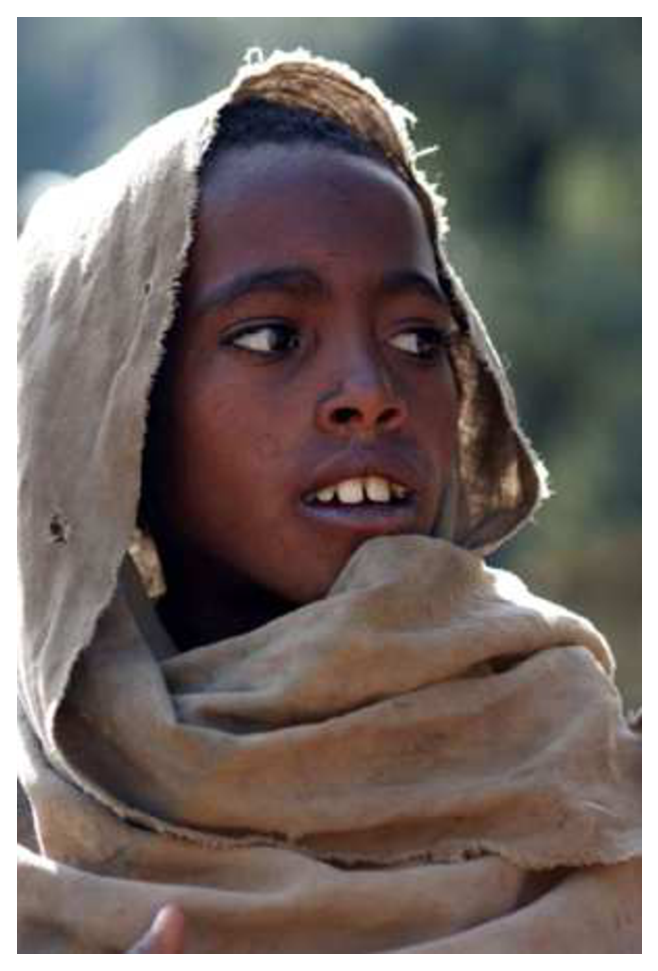
\includegraphics{etiopan.eps} \reflectbox{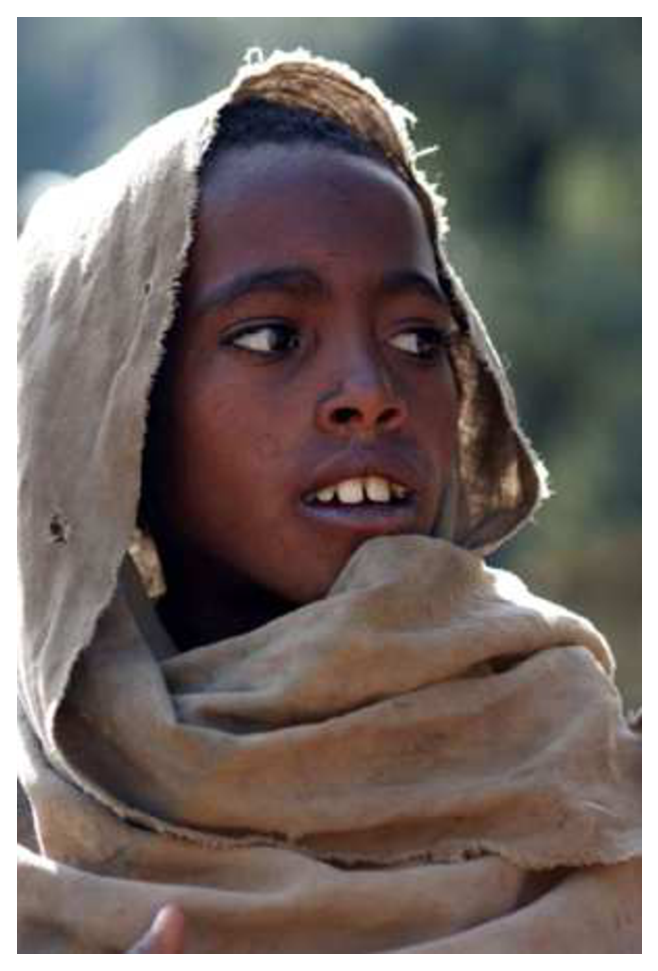
\includegraphics{etiopan.eps}} 
}
\end{center}
\caption{Malý Etiopánek a~jeho bratříček}
\label{fig:obr1}
\end{figure}

\newpage

Rozdíl mezi vektorovým\dots

\begin{figure}[ht]
\begin{center}
\scalebox{0.4}{
\includegraphics{oniisan.eps}}
\end{center}
\caption{Vektorový obrázek}
\label{fig:obr2}
\end{figure}

\dots a~bitmapovým obrázkem

\begin{figure}[ht]
\begin{center}
\scalebox{0.60}{
\includegraphics{oniisan2.eps}}
\end{center}
\caption{Bitmapový obrázek}
\label{fig:obr3}
\end{figure}

\noindent se projeví například při zvětšení. 

Odkazy (nejen ty) na obrázky \ref{fig:obr1}, \ref{fig:obr2} a~\ref{fig:obr3}, na tabulky \ref{tab:tab1} a~\ref{tab:tab2} a~také na algoritmus \ref{Algoritmus1} jsou udělány pomocí křížových odkazů. Pak je ovšem potřeba zdrojový soubor přeložit dvakrát.

Vektorové obrázky lze vytvořit i~přímo v \LaTeX u, například pomocí prostředí \texttt{\ picture}.

\begin{landscape}
\begin{figure}[ht]
\begin{picture}(700,500)
%\put(0,0) {\circle{100mm}}
%\put(700,500){\circle{100mm}}
%\put(290, 180){\circle{30mm}}
\put(57,186){\framebox(569,284)}
\put(540,414){\circle{38}}
\put(63,224) {
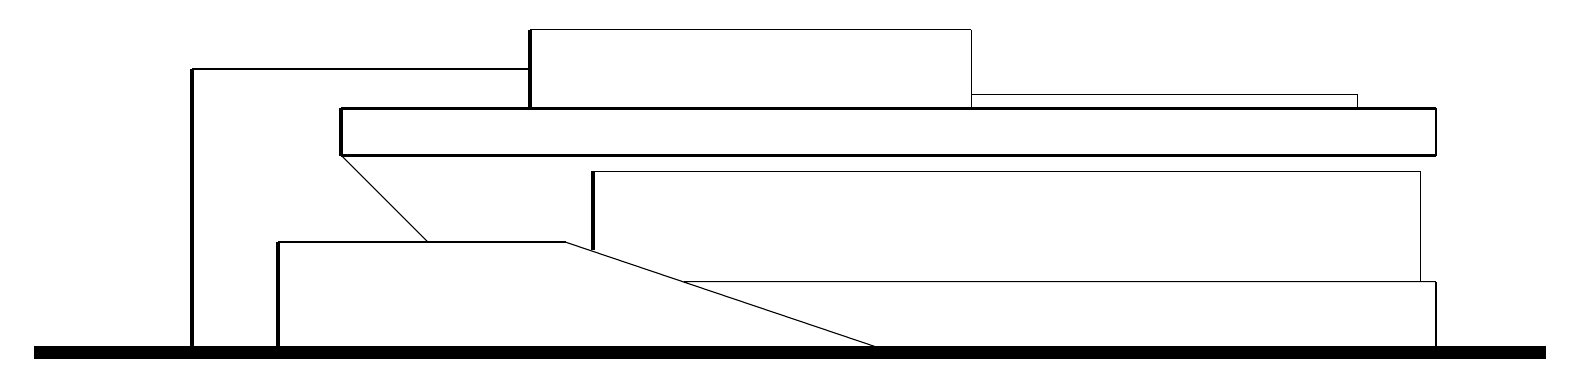
\begin{tikzpicture}
\draw [line width=1.7mm] (0,0) -- (19.2,0);
\draw [line width=0.5mm] (2,0) -- (2,3.6);
\draw (2,3.6) -- (6.3,3.6);
\draw [line width=0.5mm] 
(6.3,3.6) -- (6.3,4.1)
(6.3,3.6) -- (6.3,3.1);
\draw
(6.3,4.1) -- (11.9,4.1)
(11.9,4.1) -- (11.9,3.1)
(11.9,3.28) -- (16.8, 3.28)
(16.8, 3.28) -- (16.8, 3.1);
\draw [line width=0.5mm] (3.1,0) -- (3.1,1.4);
\draw [line width=0.3mm] (3.1,1.4) -- (6.75,1.4);
\draw 
(6.75,1.4) -- (10.9,0)
(8.25,0.9) -- (17.8,0.9);
\draw [line width=0.3mm] (17.8,0.9) -- (17.8,0);

\draw (5,1.4) -- (3.9,2.5);
\draw [line width=0.5mm] (3.9,2.5) -- (3.9,3.1);
\draw
[line width=0.3mm] (3.9,3.1) -- (17.8,3.1)
[line width=0.3mm] (3.9,2.5) -- (17.8,2.5)
[line width=0.3mm] (17.8,2.5) -- (17.8,3.1);

\draw [line width=0.5mm] (7.1,1.3) -- (7.1,2.3);
\draw
(7.1,2.3) -- (17.6,2.3)
(17.6,2.3) -- (17.6,0.9)
;
\end{tikzpicture}
}
\end{picture}
\vspace*{-7cm}
\caption{Vektorový obrázek}
\end{figure}
\end{landscape}
\restoregeometry

\end{document}